\documentclass[../../main.tex]{subfiles}
\begin{document}

\subsection*{10.6}
Una sbarra orizzontale di lunghezza $b =20\ cm$, sezione $\Sigma$, densità $\delta = 3*10^3\ \frac{kg}{m^3}$, resistività $\rho = 2 * 10^{-5}\Omega m$ può scivolare senza attrito su due guide parallele, separate dalla distanza b e inclinate di un angolo $\alpha = 30°$ rispetto al piano orizzontale.\\
Le due guide, di resistenza trascurabile, sono collegate ad un generatore di f.e.m. $\varepsilon$. Il sistema è immerso in un campo magnetico uniforme $B = 0.3\ T$ diretto secondo la verticale.\\
Calcolare il valore di $\varepsilon$ affinché la sbarra rimanga ferma, la velocità limite $v_{\infty}$ con cui la sbarra scende se il generatore viene sostituito da un corto circuito, la potenza dissipata nella sbarra quando essa scende con velocità $v_{\infty}$. (per quest'ultima domanda si assuma $\Sigma = 1\ cm^2$).\\
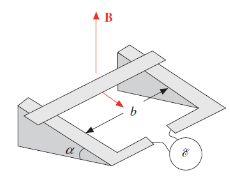
\includegraphics[]{e_10_6.png}
\subsubsection*{Formule utilizzate}
\subsubsection*{Soluzione punto a}
Sulla sbarra agiscono due forze: la forza peso e quella associata al conduttore percorso da corrente in una regione in cui è presente un campo magnetico.\\
La sbarra sarà ferma quando le componenti tangenti al piano sono uguali e opposte (con i che fluisce in verso antiorario): $\frac{\varepsilon}{R}Bb\ cos\alpha = mg\ sen\alpha$\\
Ovvero quando: $\varepsilon = R\frac{Rmg}{bB}tan\alpha = \frac{\rho b \delta b\Sigma g}{\Sigma b B}tan\alpha = \frac{\rho \delta b g}{B}tan\alpha = 0.226\ V$\\
Se il generatore viene sostituito da un corto circuito, la barra comincia a muoversi e si produce una fem che dalla regola del flusso tagliato vale $\varepsilon = Bb\ cos\alpha v$ cui corrisponde una forza "viscosa" frenante la cui componenete parallela al piano è: $F_{viscosa} = \frac{B^2b^2cos^2\alpha}{R}v$ opposta alla direzione del moto.\\
A regime, detta $v_{\infty}$ la velocità limite: $\frac{B^2b^2cos^2\alpha}{R}v_\infty = mg\ sin\alpha$\\
Da cui si calcola la velocità con cui scende la sbarra $v_\infty = \frac{mR}{b^2}\frac{g}{R^2}\frac{sin\alpha}{cos^2\alpha} = \frac{\rho \delta g}{R^2}\frac{sin\alpha}{cos^2\alpha} = 4.36\ \frac{m}{s}$\\
Infine la potenza dissipata: $P = \vec{F_g}\ \vec{v} = mg\ sin\alpha\ v_\infty = \delta \Sigma b g sin\alpha v_\infty = 1.28\ W$
\subsubsection*{Soluzione punto b}
\newpage

\end{document}